\documentclass[journal]{IEEEtran}
\usepackage[a5paper, margin=10mm, onecolumn]{geometry}
%\usepackage{lmodern} % Ensure lmodern is loaded for pdflatex
\usepackage{tfrupee} % Include tfrupee package

\setlength{\headheight}{1cm} % Set the height of the header box
\setlength{\headsep}{0mm}     % Set the distance between the header box and the top of the text

\usepackage{gvv-book}
\usepackage{gvv}
\usepackage{cite}
\usepackage{amsmath,amssymb,amsfonts,amsthm}
\usepackage{algorithmic}
\usepackage{graphicx}
\usepackage{textcomp}
\usepackage{xcolor}
\usepackage{txfonts}
\usepackage{listings}
\usepackage{enumitem}
\usepackage{mathtools}
\usepackage{gensymb}
\usepackage{comment}
\usepackage[breaklinks=true]{hyperref}
\usepackage{tkz-euclide} 
\usepackage{listings}
% \usepackage{gvv}                                        
\def\inputGnumericTable{}                                 
\usepackage[latin1]{inputenc}                                
\usepackage{color}                                            
\usepackage{array}                                            
\usepackage{longtable}                                       
\usepackage{calc}                                             
\usepackage{multirow}                                         
\usepackage{hhline}                                           
\usepackage{ifthen}                                           
\usepackage{lscape}
\begin{document}

\bibliographystyle{IEEEtran}
\vspace{3cm}

\title{10.4.4.3}
\author{EE24BTECH11017 - D.Karthik}
 \maketitle
% \newpage
% \bigskip
{\let\newpage\relax\maketitle}

\renewcommand{\thefigure}{\theenumi}
\renewcommand{\thetable}{\theenumi}
\setlength{\intextsep}{10pt} % Space between text and floats


\numberwithin{equation}{enumi}
\numberwithin{figure}{enumi}
\renewcommand{\thetable}{\theenumi}


\textbf{Question}:\\
Is it possible to design a rectangular mango grove whose length is twice its breadth, and the area is $800\, \text{m}^2$? If so, find its length and breadth.

\textbf{Solution:}\\
Let the breadth of the rectangular mango grove be $b$ meters. Then the length is $2b$ meters (as it is twice the breadth). The area of the rectangle is given as $800\, \text{m}^2$.

The relationship between the length, breadth, and area can be expressed as:
\begin{align}
    \text{Area} = \text{Length} \times \text{Breadth} \\
    800 = 2b \cdot b
\end{align}

This simplifies to a quadratic equation:
\begin{align}
    2b^2 = 800 \\
    b^2 = 400 \\
    b^2 - 400 = 0
\end{align}

The quadratic equation is:
\begin{align}
    b^2 - 400 = 0
\end{align}

We solve this quadratic equation using the eigenvalue method. Represent the quadratic equation as a matrix:
\begin{align}
    \myvec{1 & 0 \\
           0 & -400} \myvec{b^2 \\
           1} = \myvec{0 \\
           0}
\end{align}

The matrix can be decomposed to find its eigenvalues. Let the matrix $A$ be:
\begin{align}
    A = \myvec{1 & 0 \\
               0 & -400}
\end{align}

The characteristic equation for eigenvalues $\lambda$ is given by:
\begin{align}
    \det(A - \lambda I) = 0
\end{align}
where $I$ is the identity matrix. Substitute $A$ and expand:
\begin{align}
    \det\myvec{1 - \lambda & 0 \\
                0 & -400 - \lambda} = 0
\end{align}
This simplifies to:
\begin{align}
    (1 - \lambda)(-400 - \lambda) = 0
\end{align}

The eigenvalues are:
\begin{align}
    \lambda_1 = 1, \quad \lambda_2 = -400
\end{align}

To find the solution for $b$, substitute $\lambda_2$ (since $\lambda_2$ represents the quadratic term):
\begin{align}
    b^2 = -\frac{\lambda_2}{1} = 400
\end{align}

Take the square root of $b^2$:
\begin{align}
    b = \sqrt{400} = 20 \text{ meters.}
\end{align}

Substitute $b$ into the expression for the length:
\begin{align}
    \text{Length} = 2b = 2 \times 20 = 40 \text{ meters.}
\end{align}

\textbf{Conclusion:}\\
It is possible to design the mango grove with the given conditions. The dimensions are:
\begin{itemize}
    \item \textbf{Breadth:} $20\, \text{m}$
    \item \textbf{Length:} $40\, \text{m}$
\end{itemize}

\textbf{Graphical Representation:}\\
To visualize this, the rectangle can be plotted with the given dimensions, as shown below:
\begin{figure}[ht] % h: here, t: top of the page
    \centering
    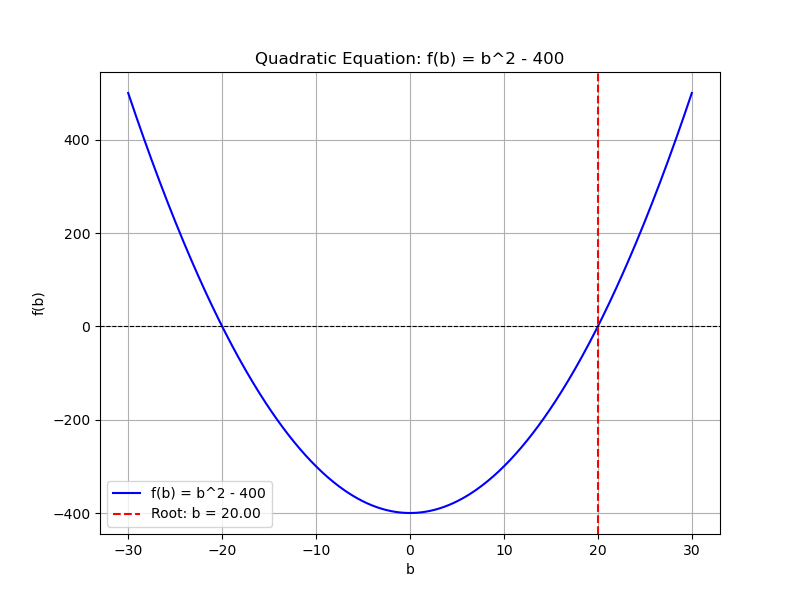
\includegraphics[width=0.5\textwidth]{figs/Figure_1.png} % Replace with your image file name
    \caption{A rectangular mango grove with length 40 m and breadth 20 m.}
    \label{fig:mango_grove}
\end{figure}
\end{document}